\documentclass[12pt,a4paper,oneside]{report}

% ==============================================================================
% PACKAGES & ACADEMIC CONFIGURATION
% ==============================================================================
\usepackage[utf8]{inputenc}
\usepackage[T1]{fontenc}
\usepackage[english]{babel}
\usepackage{geometry}
\geometry{top=2.5cm, bottom=2.5cm, left=2.5cm, right=2.5cm, headheight=15pt}
\usepackage{microtype}


\usepackage{graphicx}
\usepackage{amsmath,amssymb,amsfonts}
\usepackage{booktabs}
\usepackage{array}
\usepackage{tabularx}
\usepackage{multirow}
\usepackage{hyperref}
\usepackage{fancyhdr}
\usepackage{titlesec}
\usepackage{setspace}
\usepackage{listings}
\usepackage{xcolor}
\usepackage{caption}
\usepackage{subcaption}
\usepackage{float}
\usepackage{siunitx}
\usepackage{enumitem}
\usepackage{circuitikz}

\hypersetup{
    colorlinks=true,
    linkcolor=black,
    filecolor=magenta,      
    urlcolor=blue,
    citecolor=blue,
    pdftitle={Engineering Project Report - Giant 7-Segment Chronometer System},
    pdfauthor={Becem Ameur},
    pdfpagemode=FullScreen,
}

% Code snippet styling
\definecolor{codegreen}{rgb}{0,0.6,0}
\definecolor{codegray}{rgb}{0.5,0.5,0.5}
\definecolor{codepurple}{rgb}{0.58,0,0.82}
\definecolor{backcolour}{rgb}{0.97,0.98,0.99}

\lstdefinestyle{mystyle}{
    backgroundcolor=\color{backcolour},   
    commentstyle=\color{codegreen},
    keywordstyle=\color{blue}\bfseries,
    numberstyle=\tiny\color{codegray},
    stringstyle=\color{codepurple},
    basicstyle=\ttfamily\footnotesize,
    breakatwhitespace=false,         
    breaklines=true,                 
    captionpos=b,                    
    keepspaces=true,                 
    numbers=left,                    
    numbersep=5pt,                  
    showspaces=false,                
    showstringspaces=false,
    showtabs=false,                  
    tabsize=2
}
\lstset{style=mystyle}

% Header & Footer
\pagestyle{fancy}
\fancyhf{}
\fancyhead[L]{\nouppercase{\leftmark}}
\fancyhead[R]{ENIM -- 2025/2026}
\fancyfoot[C]{\thepage}
\renewcommand{\headrulewidth}{0.4pt}
\renewcommand{\footrulewidth}{0.4pt}

\onehalfspacing

% ==============================================================================
% DOCUMENT BEGINS
% ==============================================================================
\begin{document}

% ------------------------------------------------------------------------------
% TITLE PAGE
% ------------------------------------------------------------------------------
\begin{titlepage}
    \begin{center}
        \begin{minipage}[c]{0.2\textwidth}
            \centering
            % In your Overleaf/local project, put enim_logo.png in figures/
            \fbox{\rule{0pt}{1.8cm}\rule{1.8cm}{0pt}\textbf{\large ENIM}}
        \end{minipage}
        \hfill
        \begin{minipage}[c]{0.55\textwidth}
            \centering
            {\small \textbf{Tunisian Republic}}\\
            {\small \textbf{Ministry of Higher Education and Scientific Research}}\\
            {\small \textbf{University of Monastir}}\\
            {\small \textbf{National Engineering School of Monastir (ENIM)}}
        \end{minipage}
        \hfill
        \begin{minipage}[c]{0.2\textwidth}
            \centering
            % In your Overleaf/local project, put um_logo.png in figures/
            \fbox{\rule{0pt}{1.8cm}\rule{1.8cm}{0pt}\textbf{\large UM}}
        \end{minipage}
        
        \vspace{2.0cm}
        \rule{\linewidth}{1.4pt}\\[0.4cm]
        {\huge \textbf{Project Report}}\\[0.2cm]
        \rule{\linewidth}{1.4pt}
        
        \vspace{1.0cm}
        {\LARGE \textbf{CHRONO\_01 -- Giant 7-Segment Digital Chronometer}}\\[0.4cm]
        {\Large \textit{Comprehensive Electrical Study, High-Voltage 24V PCB Design, NPTH Rapid-Prototyping Optimization, and Dual IoT/GSM Telemetry}}
        
        \vspace{2.0cm}
        \begin{minipage}[t]{0.45\textwidth}
            \textbf{Prepared by:}\\[0.2cm]
            {\large \textbf{Becem Ameur}}\\[0.1cm]
            \textit{Engineering Student -- Electrical Engineering, $2^{nd}$ year}
        \end{minipage}
        \hfill
        \begin{minipage}[t]{0.45\textwidth}
            \begin{flushright}
                \textbf{Supervised by:}\\[0.2cm]
                {\large \textbf{Academic Supervision Team}}\\[0.1cm]
                \textit{Department of Electrical Engineering}
            \end{flushright}
        \end{minipage}
        
        \vfill
        \rule{\linewidth}{0.6pt}\\[0.2cm]
        {\textbf{Academic Year: 2025 -- 2026}}\\
        {\small National Engineering School of Monastir, University of Monastir, Tunisia}
    \end{center}
\end{titlepage}

% ------------------------------------------------------------------------------
% ABSTRACT
% ------------------------------------------------------------------------------
\pagenumbering{roman}
\setcounter{page}{2}

\chapter*{Abstract}
\addcontentsline{toc}{chapter}{Abstract}
\sloppy


\noindent\textbf{Keywords:} Embedded Systems, Custom PCB Engineering, KiCad 10, ESP32-WROVER-E, 74HC595 Shift Registers, ULN2803A Darlington Arrays, SIM800L Cellular Engine, 24V High-Power LED Displays, Non-Plated Through Hole (NPTH), Power Transient Sizing, Asynchronous Web Dashboard, Optical Diffuser.


\vspace{0.5cm}
\noindent\textbf{Context:} Large-scale outdoor athletic events, automotive rallies, and industrial timing installations require large-format numerical displays capable of delivering direct sunlight visibility, high operational robustness, and flexible multi-protocol control interfaces. Commercial turnkey timing boards are typically high in cost and utilize closed proprietary wireless systems that lack remote worldwide connectivity.

\vspace{0.4cm}
\noindent\textbf{Problem Statement:} Developing a custom, cost-effective giant chronometer system involves integrating high-voltage, high-current $24\,\text{V}$ display hardware with sensitive $3.3\,\text{V}/5\,\text{V}$ low-power IoT microcontrollers. This creates complex multidisciplinary engineering trade-offs: sinking up to $6.3\,\text{A}$ of aggregate display current without thermal degradation, buffering $2.0\,\text{A}$ transient RF bursts from GSM transceivers to prevent microcontroller brownout resets, and adapting double-sided PCB layout topologies to accommodate severe rapid-prototyping constraints (specifically Non-Plated Through Holes, track clearances $\ge 0.38\,\text{mm}$, and manual soldering access).

\vspace{0.4cm}
\noindent\textbf{Methodology:} This project report documents the comprehensive design, mathematical component sizing, CAD layout optimization, firmware development, physical chassis construction, and experimental validation of \textbf{CHRONO\_01}. The system architecture utilizes an ESP32-WROVER-E SoC hosting an asynchronous local HTTP Web server alongside a SIM800L GSM engine. A serial-to-parallel SPI cascade composed of six daisy-chained 74HC595 shift registers interfaces six ULN2803A Darlington transistor arrays to sink current from 42 individual $24\,\text{V}$ LED strip segments. The PCB layout underwent a rigorous spatial redesign under \textbf{KiCad 10}, reducing board area by $58.4\%$ (from $280\times 110\,\text{mm}$ to $160\times 80\,\text{mm}$) through a novel modular orthogonal "T-Shape" digit block geometry, teardrop pad fillets, and strategic through-hole elevation using machined-pin tulip sockets.

\vspace{0.4cm}
\noindent\textbf{Results:} The optimized PCB design achieved $100\%$ DRC validation with zero electrical violations. Physical prototyping and oscilloscope testing confirmed transient voltage ripple suppression below $80\,\text{mV}$ during GSM transmission following the integration of an engineered $1000\,\mu\text{F}$ buffer capacitor. The system was housed within a custom matte black enclosure equipped with a $3\,\text{mm}$ Opal White PMMA diffuser, achieving sharp, continuous digit illumination without optical bleed.

\vspace{0.4cm}
\noindent\textbf{Conclusion:} The final platform delivers an industrial-grade, field-deployable chronometer with hybrid local WiFi and worldwide cellular SMS control. The report concludes with detailed roadmaps for future enhancements, including pin-compatible 4G LTE-Cat1 migration and wide-input automotive power regulation.

\newpage

% ------------------------------------------------------------------------------
% DEDICATION & ACKNOWLEDGEMENTS
% ------------------------------------------------------------------------------
\chapter*{Dedication}
\addcontentsline{toc}{chapter}{Dedication}
\begin{center}
    \vspace*{3cm}
    \textit{To my beloved parents and family, for their endless sacrifices, unwavering encouragement, and profound faith in my aspirations.}\\[1cm]
    \textit{To the faculty and engineering professors of ENIM, who cultivate technical rigor, innovation, and scientific integrity.}\\[1cm]
    \textit{To all engineering students and makers who transform theoretical equations into living, tangible technology.}
\end{center}

\newpage

\chapter*{Acknowledgements}
\addcontentsline{toc}{chapter}{Acknowledgements}
The author wishes to express sincere gratitude and appreciation to:
\begin{itemize}[leftmargin=1.5cm, label=$\bullet$]
    \item \textbf{The Academic Supervision Team at the National Engineering School of Monastir (ENIM)}, for their guidance, constructive feedback, and continuous support throughout this engineering project.
    \item \textbf{The Department of Electrical Engineering}, for providing the technical curriculum, prototyping facilities, and instrumentation required for experimental verification.
    \item \textbf{The Open-Source Hardware and Software Communities} (KiCad Development Team, Espressif Systems), for delivering advanced, accessible toolchains that empower student engineering research.
    \item \textbf{Colleagues, peers, and local electronic suppliers in Tunisia} (Didactico, CoThings, Geek-Shop), for their assistance in component sourcing and rapid manufacturing coordination.
\end{itemize}

\newpage

% ------------------------------------------------------------------------------
% TABLE OF CONTENTS & LISTS
% ------------------------------------------------------------------------------
\tableofcontents
\listoffigures
\listoftables

\newpage

% ------------------------------------------------------------------------------
% LIST OF ACRONYMS
% ------------------------------------------------------------------------------
\chapter*{List of Acronyms}
\addcontentsline{toc}{chapter}{List of Acronyms}

\begin{table}[H]
\centering
\begin{tabular}{ll}
\toprule
\textbf{Acronym} & \textbf{Definition} \\
\midrule
\textbf{AC} & Alternating Current \\
\textbf{ADC} & Analog-to-Digital Converter \\
\textbf{API} & Application Programming Interface \\
\textbf{BJT} & Bipolar Junction Transistor \\
\textbf{BOM} & Bill of Materials \\
\textbf{CAD} & Computer-Aided Design \\
\textbf{CMOS} & Complementary Metal-Oxide-Semiconductor \\
\textbf{DC} & Direct Current \\
\textbf{DIP} & Dual In-line Package \\
\textbf{DRC} & Design Rule Check \\
\textbf{DRL} & Drill File (NC Excellon format) \\
\textbf{ESR} & Equivalent Series Resistance \\
\textbf{GBR} & Gerber RS-274X File Format \\
\textbf{GPIO} & General Purpose Input/Output \\
\textbf{GSM} & Global System for Mobile Communications \\
\textbf{HTTP} & Hypertext Transfer Protocol \\
\textbf{IC} & Integrated Circuit \\
\textbf{IoT} & Internet of Things \\
\textbf{LED} & Light Emitting Diode \\
\textbf{LDO} & Low Drop-Out (Linear Voltage Regulator) \\
\textbf{LTE} & Long-Term Evolution \\
\textbf{MOSFET} & Metal-Oxide-Semiconductor Field-Effect Transistor \\
\textbf{NPTH} & Non-Plated Through Hole \\
\textbf{NTP} & Network Time Protocol \\
\textbf{OTA} & Over-The-Air (Firmware Update) \\
\textbf{PCB} & Printed Circuit Board \\
\textbf{PMMA} & Poly(methyl methacrylate) / Acrylic Glass \\
\textbf{PSRAM} & Pseudo-Static Random Access Memory \\
\textbf{PTH} & Plated Through Hole \\
\textbf{PWM} & Pulse-Width Modulation \\
\textbf{REST} & Representational State Transfer \\
\textbf{RTC} & Real-Time Clock \\
\textbf{SEPIC} & Single-Ended Primary-Inductor Converter \\
\textbf{SMD} & Surface-Mount Device \\
\textbf{SMPS} & Switched-Mode Power Supply \\
\textbf{SoC} & System-on-Chip \\
\textbf{SPI} & Serial Peripheral Interface \\
\textbf{UART} & Universal Asynchronous Receiver-Transmitter \\
\textbf{VCC} & Voltage Common Collector \\
\bottomrule
\end{tabular}
\end{table}

\newpage
\pagenumbering{arabic}
\setcounter{page}{1}

% ==============================================================================
% CHAPTER 1: PROJECT CONTEXT & REQUIREMENTS
% ==============================================================================
\chapter{Project Context, Industrial Requirements and System Architecture}

\section{Introduction}
Large-format electronic timing displays and scoreboards are vital across professional athletics, vehicular rallies, public events, and industrial monitoring. The principal function of such displays is to convey high-precision chronological data across substantial distances under demanding optical and environmental conditions. 

This project, titled \textbf{CHRONO\_01}, details the complete engineering workflow involved in designing, simulating, laying out, fabricating, programming, and validating an industrial-grade 6-digit giant 7-segment chronometer ($HH:MM:SS$). The system is driven by high-intensity $24\,\text{V}$ LED strip arrays and incorporates dual wireless control modalities: a local WiFi-hosted Web dashboard and worldwide SMS cellular telemetry.

\section{Context and Motivation}
Outdoor athletic competitions—such as circuit racing, marathons, and collegiate sporting events—present stringent requirements for timing instrumentation:
\begin{enumerate}
    \item \textbf{Long-Distance Optical Legibility:} Displays must maintain crisp contrast and high luminous output under direct solar illumination ($> 50\,000\,\text{lux}$ ambient daylight), requiring high-power $24\,\text{V}$ LED bars rather than low-power discrete 5V LEDs.
    \item \textbf{Deployment Flexibility:} Operators on the track or sports field need instantaneous control via smartphone or tablet without installing proprietary native apps or relying on external internet routers.
    \item \textbf{Remote Telemetry:} For point-to-point off-road rallies or remote roadside installations, the system must execute start, stop, and split-time commands across arbitrarily long distances via cellular infrastructure.
    \item \textbf{Production Cost and Modularity:} Turnkey commercial displays often retail for thousands of dinars and utilize proprietary controller architectures. Developing an open, repairable, highly optimized custom PCB provides substantial economic and educational value.
\end{enumerate}

\section{Technical and Functional Specifications}
To establish an engineering benchmark, the requirements were formalized in Table~\ref{tab:cahier_des_charges}.

\begin{table}[H]
\centering
\caption{CHRONO\_01 Technical and Functional Specifications}
\label{tab:cahier_des_charges}
\begin{tabularx}{\textwidth}{lX}
\toprule
\textbf{Parameter} & \textbf{Specification / Requirement} \\
\midrule
\textbf{Display Format} & 6 Numerical Digits ($HH:MM:SS$) with dual colon separators ($:$) \\
\textbf{Total Segment Count} & 42 Active LED Bar Segments ($6 \text{ digits} \times 7 \text{ segments}$) \\
\textbf{Operating Voltage} & $24\,\text{V}$ DC (Main Power Bus) / $5\,\text{V}$ DC (Logic \& GSM) / $3.3\,\text{V}$ (MCU) \\
\textbf{Digit Height / Visibility} & $\approx 150 - 200\,\text{mm}$ per digit / Readable from $> 50\,\text{meters}$ \\
\textbf{Maximum Power Draw} & $\approx 45\,\text{W}$ ($24\,\text{V} @ 1.875\,\text{A}$) with all segments illuminated (\texttt{88:88:88}) \\
\textbf{Local Control Interface} & Embedded Asynchronous HTTP Web Server ($802.11\text{b/g/n}$ Soft-AP) \\
\textbf{Remote Control Interface} & Cellular SMS Telemetry via AT Command Parsing Engine \\
\textbf{PCB Form Factor} & Compact dual-layer board ($\le 160 \times 80\,\text{mm}$), single-chassis mounting \\
\textbf{Fabrication Standard} & NPTH-compatible rapid prototyping, trace width $\ge 0.38\,\text{mm}$ \\
\bottomrule
\end{tabularx}
\end{table}

\section{System Architecture and Data Flow}
The architecture is structured into four distinct physical and electrical domains:
\begin{itemize}
    \item \textbf{Power Conditioning Domain:} Accepts $24\,\text{V}$ DC from an external AC/DC SMPS or automotive boost converter, distributing $24\,\text{V}$ directly to display anodes while an on-board switching Buck converter generates a regulated $5\,\text{V}$ rail.
    \item \textbf{Central Processing Domain:} The ESP32 dual-core SoC coordinates timing, parses incoming cellular messages, hosts the web dashboard, and shifts binary display frames.
    \item \textbf{Logic and Driver Domain:} Six cascaded 74HC595 shift registers serialize 48 bits of segment data, which are level-shifted and current-sunk by six ULN2803A Darlington driver ICs.
    \item \textbf{Display Enclosure Domain:} 42 precision-cut 24V LED strip bars housed behind optical light baffles and an opal white acrylic diffusion panel.
\end{itemize}

\begin{figure}[H]
\centering
% \includegraphics[width=0.88\textwidth]{figures/system_block_diagram.png}
\fbox{\parbox{0.9\textwidth}{
\centering
\vspace{0.4cm}
\textbf{\large Complete Hardware Architecture and Domain Partitioning}\\[0.4cm]
\begin{tabular}{ccccc}
\fbox{\parbox{2.4cm}{\centering\textbf{Power Source}\\230V AC / 12V DC}} & $\xrightarrow{24\text{V}}$ & \fbox{\parbox{3.0cm}{\centering\textbf{PCB Power Bus}\\$C_2 = 100\mu\text{F} / 50\text{V}$}} & $\xrightarrow{24\text{V}}$ & \fbox{\parbox{3.2cm}{\centering\textbf{42x LED Segments}\\Common Anode (+24V)}} \\
 & & $\Big\downarrow$ & & $\Big\uparrow \text{Sinking (-)}$ \\
 & & \fbox{\parbox{3.0cm}{\centering\textbf{Buck LM2596}\\$24\text{V} \rightarrow 5\text{V}$ Reg.}} & $\xrightarrow{5\text{V}}$ & \fbox{\parbox{3.2cm}{\centering\textbf{6x ULN2803A}\\Darlington Sinks}} \\
 & & $\Big\downarrow 5\text{V} + C_1 (1000\mu\text{F})$ & & $\Big\uparrow \text{Logic Lines}$ \\
\fbox{\parbox{2.4cm}{\centering\textbf{User Interfaces}\\WiFi Web / SMS}} & $\longleftrightarrow$ & \fbox{\parbox{3.0cm}{\centering\textbf{ESP32-WROVER}\\Dual-Core Controller}} & $\xrightarrow[\text{Data, Clk, Lat}]{\text{SPI Bus}}$ & \fbox{\parbox{3.2cm}{\centering\textbf{6x 74HC595}\\Cascaded Registers}} \\
\end{tabular}
\vspace{0.4cm}
}}
\caption{CHRONO\_01 Detailed System Architecture and Inter-Domain Signal Paths}
\label{fig:macro_arch}
\end{figure}

% ==============================================================================
% CHAPTER 2: PRELIMINARY STUDY & HARDWARE SIZING
% ==============================================================================
\chapter{Preliminary Comparative Study and Hardware Sizing}

\section{Introduction}
Designing an industrial embedded system requires evaluating alternative components to identify optimal trade-offs between performance, reliability, ease of integration, and procurement feasibility. This chapter presents the comparative study that justified our component selections, followed by the rigorous mathematical sizing of the electrical network.

\section{Component Selection and Trade-Off Analysis}

\subsection{Microcontroller Unit (MCU) Benchmarking}
Three candidate processing platforms were evaluated and compared against the chosen Espressif \textbf{ESP32-WROVER-E}: the 8-bit ATmega328P (widely used in Arduino Uno boards) and the 32-bit ARM Cortex-M4 STM32F401.

\begin{table}[H]
\centering
\small
\caption{Microcontroller Benchmarking Matrix}
\label{tab:mcu_comparison}
\begin{tabularx}{\textwidth}{>{\raggedright\arraybackslash}X c c >{\raggedright\arraybackslash}p{3.8cm}}
\toprule
\textbf{Feature / Parameter} & \textbf{ATmega328P} & \textbf{STM32F401} & \textbf{ESP32-WROVER-E} (\textit{Selected}) \\
\midrule
Architecture & 8-bit AVR & 32-bit ARM M4 & \textbf{32-bit Dual-Core Xtensa} \\
Clock Frequency & $16\,\text{MHz}$ & $84\,\text{MHz}$ & \textbf{$240\,\text{MHz}$} \\
SRAM & $2\,\text{KB}$ & $96\,\text{KB}$ & \textbf{$520\,\text{KB} + 8\,\text{MB PSRAM}$} \\
Flash Memory & $32\,\text{KB}$ & $512\,\text{KB}$ & \textbf{$4\,\text{MB}$ SPI Flash} \\
Integrated Wi-Fi & None & None & \textbf{$802.11\text{b/g/n}$ Native} \\
Integrated Bluetooth & None & None & \textbf{BLE 4.2 Native} \\
Hardware UART Channels & 1 & 3 & \textbf{3 Hardware UARTs} \\
Asynchronous Web Server & Unfeasible & Complex (Shield) & \textbf{Native AsyncTCP HTTP} \\
Dual-Core Parallelism & No & No & \textbf{Yes (Core0 + Core1)} \\
Unit Cost (Tunisia, 2025/2026) & $\approx 15\,\text{TND}$ & $\approx 35\,\text{TND}$ & \textbf{$\approx 32\,\text{TND}$} \\
\bottomrule
\end{tabularx}
\end{table}

\noindent\textbf{Decision Rationale:} The ESP32-WROVER-E was selected as the only platform capable of natively hosting both a dual-core parallel real-time execution environment and integrated WiFi without any external shields. Its dual-core architecture allows Core 0 to handle the network stack (Soft-AP and asynchronous HTTP Web server) while Core 1 executes deterministic $1\,\text{ms}$ chronometer tick counting, SPI display frame updates, and UART GSM AT command parsing without timing jitter. The ATmega328P was disqualified by its lack of WiFi and insufficient SRAM for HTML page hosting. The STM32F401, while computationally capable, would require an external WiFi module (ESP8266 or W5500 Ethernet shield), adding cost and PCB footprint.

% ==============================================================================
% ECONOMIC ANALYSIS SECTION
% ==============================================================================
\section{Economic Cost Analysis: Custom Development vs.~Commercial Purchase}

\subsection{Overview}
A critical engineering decision at the project outset was determining whether to design and build a custom chronometer or acquire an equivalent commercial product. This section presents the detailed financial comparison between the cost of the custom \textbf{CHRONO\_01} platform and the market price of equivalent turnkey commercial timing systems.

\subsection{CHRONO\_01 Bill of Materials Cost (Detailed Breakdown)}
All components were sourced from Tunisian suppliers (Didactico Tunis, CoThings, Geek-Shop.tn, local Sfax electronic shops) with 2025/2026 pricing.

\begin{table}[H]
\centering
\small
\caption{Detailed Component Cost Breakdown for CHRONO\_01 (Tunisian Market)}
\label{tab:cost_bom}
\begin{tabularx}{\textwidth}{>{\raggedright\arraybackslash}X c r r}
\toprule
\textbf{Component / Item} & \textbf{Qty} & \textbf{Unit Price (TND)} & \textbf{Subtotal (TND)} \\
\midrule
\multicolumn{4}{l}{\textit{\textbf{Electronic Components}}} \\
ESP32-WROVER-E Development Board & 1 & 32.00 & 32.00 \\
74HC595 Shift Register IC (DIP-16) & 6 & 2.50 & 15.00 \\
Machined Tulip DIP-16 Sockets (paire) & 6 & 1.80 & 10.80 \\
ULN2803A Darlington Array IC (DIP-18) & 6 & 3.20 & 19.20 \\
Machined Tulip DIP-18 Sockets (paire) & 6 & 2.00 & 12.00 \\
SIM800L GSM Module + SIM Card & 1 & 45.00 & 45.00 \\
LM2596 Buck Step-Down Module ($24\text{V}\to5\text{V}$) & 1 & 12.00 & 12.00 \\
Electrolytic Capacitor $1000\,\mu\text{F}$/16V (low-ESR) & 2 & 2.50 & 5.00 \\
Electrolytic Capacitor $100\,\mu\text{F}$/50V & 2 & 1.50 & 3.00 \\
Ceramic Capacitors $100\,\text{nF}$/50V (pack of 20) & 1 & 3.00 & 3.00 \\
Resistor $2.4\,\text{k}\Omega$ / $0.25\,\text{W}$ (pack of 10) & 1 & 1.00 & 1.00 \\
LED indicator 5mm Red & 2 & 0.50 & 1.00 \\
JST-XH 8-Pin Male Headers (x10 pack) & 1 & 8.00 & 8.00 \\
2-Pin Screw Terminal ($5.08\,\text{mm}$) & 2 & 1.20 & 2.40 \\
Pin Headers male/female $2.54\,\text{mm}$ (various) & -- & -- & 5.00 \\
Micro-USB Cable for programming & 1 & 8.00 & 8.00 \\
\midrule
\multicolumn{4}{l}{\textit{\textbf{PCB Fabrication}}} \\
PCB Chemical Etching (Artisan local custom board) & 1 & 120.00 & \textbf{120.00} \\
\midrule
\multicolumn{4}{l}{\textit{\textbf{Display Mechanical Structure}}} \\
24V COB LED Strip (High Density, 5m roll) & 2 & 35.00 & 70.00 \\
24V DC / 2.5A SMPS Power Supply (S-60-24) & 1 & 55.00 & 55.00 \\
Forex (PVC) Board $5\,\text{mm}$, $60\times40\,\text{cm}$ & 2 & 18.00 & 36.00 \\
Opal PMMA Acrylic Sheet $3\,\text{mm}$, $60\times40\,\text{cm}$ & 1 & 45.00 & 45.00 \\
Black Matte Paint + Primer & 1 & 15.00 & 15.00 \\
Wiring (8-conductor ribbon cable, 3m) & 2 & 10.00 & 20.00 \\
Heat Shrink Tubing + Cable Ties & -- & -- & 8.00 \\
Screws, Nuts, Standoffs (assorted) & -- & -- & 10.00 \\
\midrule
\multicolumn{4}{l}{\textit{\textbf{Miscellaneous and Consumables}}} \\
Solder Wire, Flux, Soldering Iron Tips & -- & -- & 25.00 \\
Multimeter probes replacement & -- & -- & 12.00 \\
Prototyping Breadboard and jumper wires & -- & -- & 20.00 \\
Shipping / Transport (Sfax -- Tunis round trip) & -- & -- & 60.00 \\
\midrule
\textbf{TOTAL PROJECT INVESTMENT} & & & \textbf{$\approx 740.00$ TND} \\
\bottomrule
\end{tabularx}
\end{table}

\subsection{Equivalent Commercial Product Market Pricing}
An equivalent commercial 6-digit giant 7-segment chronometer system with wireless remote control is offered by several specialized manufacturers. Based on market research conducted in 2025/2026:

\begin{table}[H]
\centering
\small
\caption{Comparative Market Pricing of Commercial Equivalent Timing Systems}
\label{tab:cost_commercial}
\begin{tabularx}{\textwidth}{>{\raggedright\arraybackslash}X c c}
\toprule
\textbf{Commercial Product Category} & \textbf{Typical Price (EUR)} & \textbf{Approx. Price (TND)} \\
\midrule
Portable Race Clock / Sports Timer (amateur, WiFi only) & 250 -- 500 EUR & 850 -- 1,700 TND \\
Professional Race Chronometer with GSM + WiFi (Bodet, Stramatel) & 900 -- 1,500 EUR & 3,060 -- 5,100 TND \\
Giant 7-Segment Custom LED Scoreboard (per digit, installed) & 350 -- 800 EUR/digit & 1,190 -- 2,720 TND/digit \\
6-Digit Installed Scoreboard System (Turnkey) & 2,500 -- 6,000 EUR & 8,500 -- 20,400 TND \\
Chinese OEM Equivalent (AliExpress, import + customs + shipping) & 400 -- 900 USD & 1,340 -- 3,010 TND \\
\bottomrule
\end{tabularx}
\end{table}
\small\textit{Note: Conversion rate applied: 1 EUR $\approx$ 3.40 TND; 1 USD $\approx$ 3.35 TND (Banque Centrale de Tunisie).}
\normalsize

\subsection{Economic Comparison Summary}
\begin{table}[H]
\centering
\small
\caption{Final Economic Comparison: CHRONO\_01 vs. Commercial Equivalents}
\label{tab:cost_summary}
\begin{tabular}{lcc}
\toprule
\textbf{Criterion} & \textbf{CHRONO\_01 (This Project)} & \textbf{Commercial Equivalent} \\
\midrule
\textbf{Total Investment} & $\approx \textbf{740 TND}$ & 3,060 -- 20,400 TND \\
\textbf{Cost Saving} & \multicolumn{2}{c}{\textbf{76\% -- 96\% less expensive}} \\
\textbf{WiFi Control} & $\checkmark$ Native Soft-AP & $\checkmark$ (some models) \\
\textbf{GSM SMS Telemetry} & $\checkmark$ SIM800L Included & $\checkmark$ (premium models only) \\
\textbf{Digit Height / Visibility} & $\approx 180\,\text{mm}$ / $> 50\,\text{m}$ & $150 - 200\,\text{mm}$ / $> 50\,\text{m}$ \\
\textbf{Repairability} & $\checkmark$ Full open-source schematics & $\times$ Proprietary, void warranty \\
\textbf{Customizability} & $\checkmark$ Complete firmware control & $\times$ Locked to vendor app \\
\textbf{OTA Firmware Updates} & $\checkmark$ Arduino OTA capable & $\times$ Not available \\
\textbf{Technical Knowledge Gained} & $\checkmark$ Complete engineering cycle & $\times$ None (plug-and-play) \\
\bottomrule
\end{tabular}
\end{table}

This analysis clearly demonstrates that the custom-designed \textbf{CHRONO\_01} platform achieves an investment cost that is \textbf{4.1 to 27 times lower} than equivalent turnkey commercial products available on the international market. Beyond the direct financial advantage, the custom solution offers complete repairability, open-source firmware customizability, and full technical ownership that no commercial vendor can match.


\subsection{I/O Expansion Topology: 74HC595 vs. I2C Expanders vs. Dedicated LED Drivers}
Controlling 42 independent segment lines requires expanding the limited GPIO count of the microcontroller. Three expansion strategies were analyzed:
\begin{enumerate}
    \item \textbf{I2C Expanders (MCP23017 / PCF8574):} While versatile, I2C expanders introduce bus addressing overhead, limited transmission bandwidth ($400\,\text{kHz}$ Fast Mode), and susceptibility to bus lockups under high electrical noise.
    \item \textbf{Dedicated Matrix Drivers (MAX7219):} Designed for common-cathode low-voltage matrix displays; they cannot directly handle common-anode $24\,\text{V}$ multi-LED strip segments without auxiliary level-shifting buffers.
    \item \textbf{Serial-to-Parallel Shift Registers (74HC595):} A synchronous SPI-like peripheral. Daisy-chaining six ICs requires only 3 digital lines ($\text{DATA}$, $\text{CLOCK}$, $\text{LATCH}$). Data shifting occurs at clock rates up to $25\,\text{MHz}$, permitting instantaneous display frame updates ($< 5\,\mu\text{s}$). The 74HC595 was chosen for its low cost, robust noise immunity, and simple serial cascade geometry.
\end{enumerate}

\subsection{Power Driver Topology: ULN2803A vs. Discrete MOSFETs}
To switch $24\,\text{V}$ power through 42 segments drawing up to $150\,\text{mA}$ each:
\begin{itemize}
    \item \textbf{Discrete N-Channel MOSFETs (e.g., 2N7002 / AO3400):} Requires 42 separate transistors plus 42 gate pull-down resistors and 42 gate protection resistors ($126\text{ discrete components}$), resulting in unmanageable PCB trace density.
    \item \textbf{ULN2803A Darlington Arrays:} Integrates eight NPN Darlington pairs in an 18-pin DIP package, complete with internal $2.7\,\text{k}\Omega$ base resistors compatible with $3.3\,\text{V}/5\,\text{V}$ CMOS logic and integrated transient clamp diodes. Six ULN2803A ICs satisfy the entire 42-segment demand with superior packaging efficiency.
\end{itemize}

\begin{figure}[H]
\centering
\begin{circuitikz}[scale=0.9, transform shape]
    % Input from 74HC595
    \draw (0,0) node[left] {74HC595 Pin $Q_n$} 
          to[R, l=$2.7\,\text{k}\Omega$, o-*] (2.2,0)
          -- (2.6,0) node[npn, anchor=B] (Q1) {};
    
    % Darlington Q2 stage
    \draw (Q1.E) -- (3.8,-0.75) node[npn, anchor=B] (Q2) {};
    
    % Emitter ground
    \draw (Q2.E) node[ground] {};
    
    % Common Collector tie
    \draw (Q1.C) -- (3.8,0.75) -- (Q2.C);
    \draw (3.8,0.75) -- (4.8,0.75) node[right] {ULN Output $O_n$}
          to[short, *-o] (5.2,0.75);
          
    % 24V LED load
    \draw (5.2,0.75) to[R, l=24V LED Segment] (5.2,3.0)
          node[above] {$+24\,\text{V}$ Rail};
\end{circuitikz}
\caption{Internal Schematic of a Single ULN2803A Darlington Sinking Channel}
\label{fig:uln_darlington}
\end{figure}

\section{Mathematical Sizing and Electrical Engineering Calculations}

\subsection{\texorpdfstring{GSM Buffer Reservoir Sizing ($C_1$)}{GSM Buffer Reservoir Sizing (C1)}}

The SIM800L cellular transceiver transmits in bursts according to the 2G GSM TDMA standard. During RF burst intervals, the module consumes a peak pulse current $I_{\text{peak}} = 2.0\,\text{A}$ for a slot duration of $\Delta t = 577\,\mu\text{s}$ ($1/8\text{th of a GSM frame}$).
If the voltage on the SIM800L supply line droops by more than $\Delta V_{\text{max}} = 0.4\,\text{V}$ (dropping below $3.7\,\text{V}$ from a nominal $4.1\,\text{V}$ rail), the internal brownout detector resets the module.

The theoretical capacitance required to supply this total charge deficit $\Delta Q$ is derived from the fundamental charge equation:
\begin{equation}
\Delta Q = I_{\text{peak}} \cdot \Delta t = C_1 \cdot \Delta V
\end{equation}
Rearranging for $C_1$:
\begin{equation}
C_1 = \frac{I_{\text{peak}} \cdot \Delta t}{\Delta V_{\text{max}}} = \frac{2.0\,\text{A} \times 577 \times 10^{-6}\,\text{s}}{0.4\,\text{V}} = \frac{1.154 \times 10^{-3}\,\text{C}}{0.4\,\text{V}} = 2885\,\mu\text{F}
\label{eq:cap_math}
\end{equation}
In practical operation, the LM2596 switched-mode power supply continuously supplies current at a switching frequency of $150\,\text{kHz}$, replenishing charge during the pulse. Accounting for this active source current ($I_{\text{buck}} \approx 0.8\,\text{A}$), the net discharge current is $I_{\text{net}} = 1.2\,\text{A}$, yielding:
\begin{equation}
C_{1(\text{effective})} = \frac{1.2\,\text{A} \times 577 \times 10^{-6}\,\text{s}}{0.4\,\text{V}} = 1731\,\mu\text{F}
\end{equation}
To achieve high transient stability with low Equivalent Series Resistance (ESR), a high-quality radial electrolytic capacitor of \textbf{$1000\,\mu\text{F}$ / $16\,\text{V}$} (or $2200\,\mu\text{F}$) was positioned immediately adjacent ($< 5\,\text{mm}$) to the SIM800L power pins.

\subsection{\texorpdfstring{Buck Regulator Input Decoupling Sizing ($C_2$)}{Buck Regulator Input Decoupling Sizing (C2)}}
The LM2596 DC-DC step-down converter operates in continuous conduction mode at $f_s = 150\,\text{kHz}$, corresponding to a switching period $T_s = 6.67\,\mu\text{s}$. The average input current at maximum load ($P_{\text{load}} \approx 10\,\text{W}$) is:
\begin{equation}
I_{\text{in(avg)}} = \frac{V_{\text{out}} \cdot I_{\text{out}}}{\eta \cdot V_{\text{in}}} = \frac{5\,\text{V} \times 2.0\,\text{A}}{0.85 \times 24\,\text{V}} \approx 0.49\,\text{A}
\end{equation}
To restrict the input voltage ripple to $\Delta V_{\text{in}} \le 100\,\text{mV}$:
\begin{equation}
C_2 = \frac{I_{\text{in(avg)}} \cdot D \cdot (1 - D)}{f_s \cdot \Delta V_{\text{in}}}
\end{equation}
Where duty cycle $D = \frac{V_{\text{out}}}{V_{\text{in}}} = \frac{5}{24} \approx 0.208$:
\begin{equation}
C_2 = \frac{0.49 \times 0.208 \times (1 - 0.208)}{150 \times 10^3 \times 0.1} = \frac{0.0807}{15000} \approx 5.38\,\mu\text{F}
\end{equation}
Accounting for parasitic trace inductance from long external power cables and automotive alternator transients, an engineering safety multiplier of $> 15\times$ is applied, establishing a standard industrial value of \textbf{$100\,\mu\text{F}$ / $50\,\text{V}$}.

\subsection{Current Limiting Resistor Sizing for Power LED ($R_1$)}
A high-efficiency 5mm Red LED ($D_1$) indicates active $24\,\text{V}$ DC power. For a forward voltage drop $V_f = 2.0\,\text{V}$ and nominal target current $I_{\text{target}} = 10\,\text{mA}$:
\begin{equation}
R_1 = \frac{V_{CC} - V_f}{I_{\text{target}}} = \frac{24\,\text{V} - 2.0\,\text{V}}{0.010\,\text{A}} = \frac{22\,\text{V}}{0.010\,\text{A}} = 2200\,\Omega = 2.2\,\text{k}\Omega
\end{equation}
When substituting a standard available $2.4\,\text{k}\Omega$ metal-film resistor:
\begin{equation}
I_{\text{actual}} = \frac{22\,\text{V}}{2400\,\Omega} = 9.16\,\text{mA}
\end{equation}
The power dissipated across the resistor is:
\begin{equation}
P_{R1} = I_{\text{actual}}^2 \cdot R_1 = (0.00916\,\text{A})^2 \times 2400\,\Omega = 0.201\,\text{W}
\end{equation}
Because $P_{R1} < 0.25\,\text{W}$, a standard $1/4\,\text{W}$ through-hole resistor operates comfortably within thermal limits ($80.4\%$ load).

\subsection{PCB Copper Trace Width Sizing (IPC-2152 Standard)}
The primary $24\,\text{V}$ bus supplies 6 digits. With all 42 segments lit (\texttt{88:88:88}), total current reaches:
\begin{equation}
I_{\text{total}} = 42 \times 40\,\text{mA} = 1.68\,\text{A}
\end{equation}
According to the IPC-2152 design standard for an internal temperature rise $\Delta T \le 10^\circ\text{C}$ on $1\,\text{oz}$ copper foil ($35\,\mu\text{m}$ thickness):
\begin{itemize}
    \item Signal traces ($< 20\,\text{mA}$): Width set to $0.38 - 0.45\,\text{mm}$ (exceeding electrical need to satisfy fabrication rules).
    \item Power traces ($24\,\text{V}$, $5\,\text{V}$, $\text{GND}$ carrying up to $2.0\,\text{A}$): Width set to $\mathbf{0.80 - 1.00\,\text{mm}}$, ensuring low impedance and negligible voltage drop ($< 15\,\text{mV}$).
\end{itemize}

% ==============================================================================
% CHAPTER 3: PCB CAD & RAPID-PROTOTYPING OPTIMIZATION
% ==============================================================================
\chapter{PCB Computer-Aided Design and Manufacturing Optimization}

\section{Introduction}
Transforming an electrical schematic into a manufacturable, noise-immune printed circuit board requires meticulous spatial planning, layer budgeting, and adherence to fabrication constraints. This chapter documents the complete CAD optimization workflow in \textbf{KiCad 10} that reduced board area by $58.4\%$ while resolving the challenges of non-plated rapid prototyping.

\section{Schematic Capture and Hierarchical Architecture}
The electrical schematic was captured in \textbf{KiCad 10} using structured netlists and bus definitions. The circuit was partitioned into four functional subsystems:
\begin{enumerate}
    \item \textbf{Power Conditioning Block:} Reverse polarity protection, input bulk filtering ($C_2$), LM2596 buck breakout footprint, and $5\,\text{V}$ output buffer stage ($C_1$).
    \item \textbf{Processing Block:} ESP32-WROVER-E footprint (38-pin dual-row) with decoupling capacitors and hardware UART breakout ($Conn\_01x07$) for GSM expansion.
    \item \textbf{Serial Shift Chain Block:} Six 74HC595 shift registers configured in daisy-chain ($Q_{7S} \rightarrow DS$) with individual $100\,\text{nF}$ ceramic decoupling capacitors positioned directly across VCC (Pin 16) and GND (Pin 8).
    \item \textbf{Power Sinking Bank:} Six ULN2803A Darlington ICs paired with JST-XH 8-pin shrouded headers ($J_2 - J_7$).
\end{enumerate}

\begin{figure}[H]
\centering
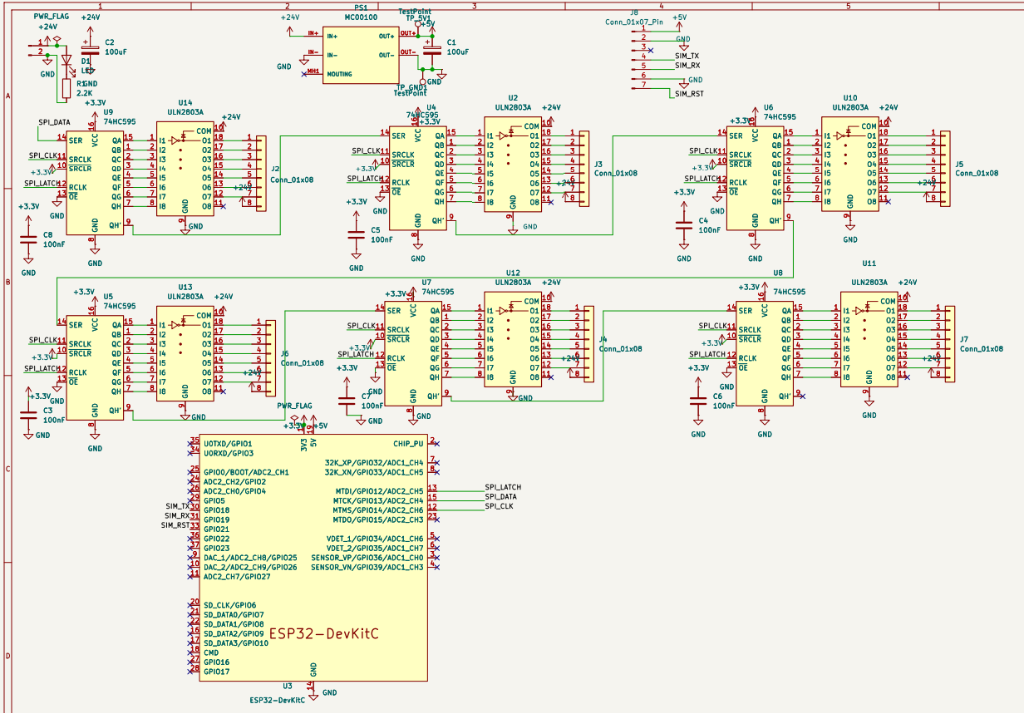
\includegraphics[width=\textwidth]{figures/kicad_schematic.png}
\caption{Complete Electrical Schematic of CHRONO\_01 in KiCad 10}
\label{fig:kicad_sch}
\end{figure}


\section{Spatial Optimization and Layout Compaction}
The preliminary prototype layout positioned all components in an extended linear row spanning $280 \times 110\,\text{mm}$ ($308\,\text{cm}^2$). This arrangement resulted in excessive trace lengths ($> 220\,\text{mm}$ for SPI lines), high electromagnetic susceptibility, and high manufacturing costs.

\begin{table}[H]
\centering
\small
\caption{PCB Spatial and Electrical Optimization Metrics}
\label{tab:pcb_opt}
\begin{tabularx}{\textwidth}{>{\raggedright\arraybackslash}X c c >{\raggedright\arraybackslash}p{4.2cm}}
\toprule
\textbf{Design Parameter} & \textbf{Initial Prototype} & \textbf{Optimized Redesign} & \textbf{Quantitative Gain} \\
\midrule
Board Outline & $280 \times 110\,\text{mm}$ & $160 \times 80\,\text{mm}$ & \textbf{-58.4\% Board Area} \\
SPI Bus Total Trace Length & $\approx 640\,\text{mm}$ & $\approx 180\,\text{mm}$ & \textbf{-71.8\% Parasitic Loop} \\
Signal Track Width & $0.25\,\text{mm}$ & $0.38 - 0.45\,\text{mm}$ & \textbf{+52\% Robustness} \\
Power Track Width & $0.60\,\text{mm}$ & $0.80 - 1.00\,\text{mm}$ & \textbf{+33\% Current Sinking} \\
Via Pad Diameter & $0.80\,\text{mm}$ & $1.60\,\text{mm}$ & \textbf{+100\% Annular Area} \\
Via Drill Diameter & $0.30\,\text{mm}$ & $0.80\,\text{mm}$ & \textbf{+166\% Drill Clearance} \\
Digit Block Layout & Linear spread & Orthogonal "T-Shape" & \textbf{Planar zero-crossing} \\
\bottomrule
\end{tabularx}
\end{table}

\section{The Modular Orthogonal "T-Shape" Digit Block}
To eliminate the dense trace crossings between the 74HC595 outputs and ULN2803A inputs, an orthogonal **"T-Shape" geometry** was developed:
\begin{itemize}
    \item The 74HC595 IC is placed **horizontally** along the top row, with its lower pins (Q0--Q7) facing south.
    \item The ULN2803A Darlington IC is placed **vertically** immediately below it.
    \item The JST-XH 8-pin connector is placed vertically adjacent to the ULN2803A.
\end{itemize}
This arrangement creates an uncrossed, parallel "waterfall" fanout where each 74HC595 output enters its corresponding ULN2803A input on a single layer without requiring vias.

\begin{figure}[H]
\centering
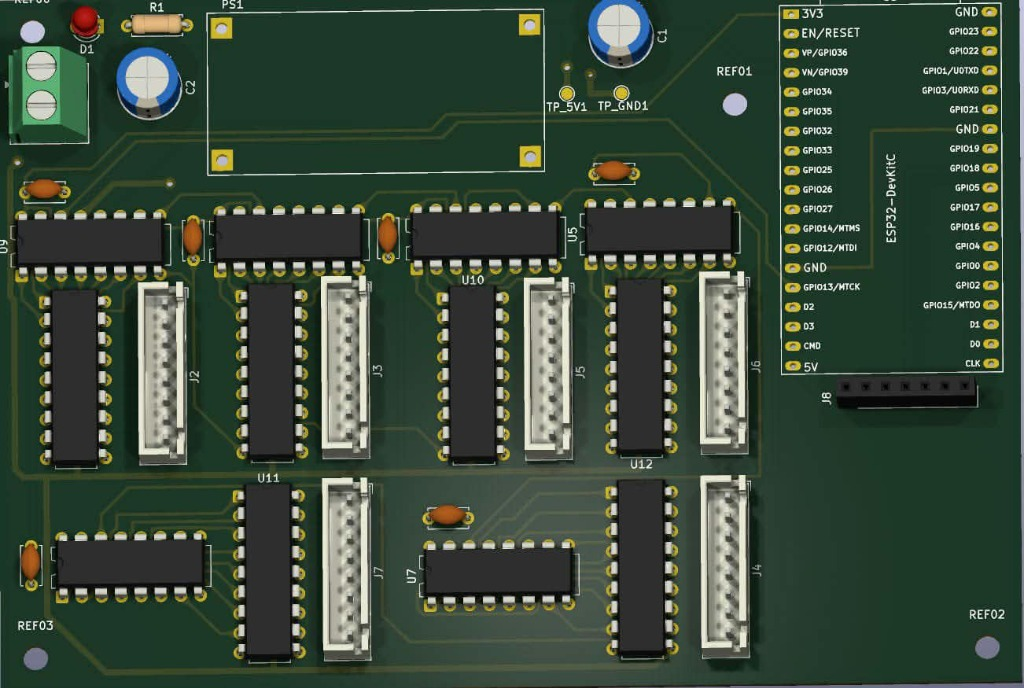
\includegraphics[width=0.92\textwidth]{figures/pcb_3d_render.jpg}
\caption{Photorealistic 3D CAD Render of the Populated CHRONO\_01 PCB in KiCad 10, Illustrating the Modular Orthogonal T-Shape Digit Architecture and Elevated Tulip Sockets}
\label{fig:pcb_3d}
\end{figure}

\section{Adapting to Non-Plated Through Hole (NPTH) Manufacturing}
Rapid-prototyping PCB milling and chemical etching laboratories frequently operate without chemical electroplating baths. Under **Non-Plated Through Hole (NPTH)** manufacturing:
\begin{itemize}
    \item Drilled holes consist of bare fiberglass substrate; there is no cylindrical copper barrel inside the hole to connect the top copper layer ($\text{F.Cu}$) to the bottom copper layer ($\text{B.Cu}$).
    \item Electrical continuity between layers relies strictly on soldering through-hole component pins or wire jumpers on both sides of the board.
\end{itemize}

\subsection{Soldering Accessibility and the "Tulip" Socket Solution}
Standard low-cost flat DIP sockets sit directly against the top PCB surface, making it impossible to insert a soldering iron tip to solder top-layer copper pads ($\text{F.Cu}$).

To solve this without redesigning the entire board into a single layer, **Machined-Pin "Tulip" DIP Sockets** were adopted. These sockets feature cylindrical machined pins with built-in metal standoff collars that suspend the plastic body $1.0\,\text{mm}$ above the PCB surface. This provides full $360^\circ$ optical and physical access for fine-tip soldering irons, allowing top-layer traces ($\text{F.Cu}$) to bond to component pins.

\subsection{Teardrop Fillet Integration}
Under artisanal mechanical drilling, mechanical spindle runout ($e \approx 0.2\,\text{mm}$) can cause drill bit misalignment, risking annular ring breakout (severing the trace-to-pad junction). 
To prevent this, **Teardrop Fillets** were computed and added across all pads and vias in KiCad. The teardrop adds a tangential copper flare that reinforces the junction mechanically and guarantees electrical continuity even under significant drill offset.



\subsection{Gerber Export and Unified Excellon Drill Generation}
During initial manufacturing submissions, the automated CAM software rejected the fabrication archive because KiCad separated drills into \texttt{chrono-PTH.drl} and \texttt{chrono-NPTH.drl}. The CAM parser interpreted the \texttt{-PTH} tag as a requirement for electroplating.
The issue was resolved by activating the **Unified Drill File** option in KiCad's NC Drill generator (\textit{"Merge plated and non-plated holes into one file"}), producing a single consolidated \texttt{.drl} file accepted by the manufacturer.

% ==============================================================================
% CHAPTER 4: SYSTEM REALIZATION, FIRMWARE & VALIDATION
% ==============================================================================
\chapter{System Realization, Firmware and Validation}

\section{Mechanical Construction and LED Strip Segmentation}
The physical chronometer panel was engineered using a high-contrast multi-layer structure:
\begin{enumerate}
    \item \textbf{Backplate Substrate:} A rigid $5\,\text{mm}$ Forex (expanded PVC) sheet painted in matte black to maximize optical contrast.
    \item \textbf{LED Strip Bar Array:} High-efficiency $24\,\text{V}$ SMD 2835 LED strips were precision-cut into 42 segments ($12\,\text{cm}$ length per segment, containing 6 LEDs in series per cut).
    \item \textbf{Wiring Harness:} Each digit groups the 7 positive terminals into a single $+24\,\text{V}$ Common Anode line, while the 7 negative cathode lines are routed through an 8-conductor ribbon cable terminated with a JST-XH connector.
\end{enumerate}


\begin{figure}[H]
\centering
\fbox{\parbox{0.82\textwidth}{
\centering
\vspace{0.3cm}
\textbf{\large 7-Segment Bar Layout and JST-XH Pin Mapping}\\[0.3cm]
\begin{tabular}{cc}
\parbox{0.35\textwidth}{\centering
\texttt{\ \ --- A --- \ }\\
\texttt{|\ \ \ \ \ \ \ |}\\
\texttt{F\ \ \ \ \ \ \ B}\\
\texttt{|\ \ \ \ \ \ \ |}\\
\texttt{\ \ --- G --- \ }\\
\texttt{|\ \ \ \ \ \ \ |}\\
\texttt{E\ \ \ \ \ \ \ C}\\
\texttt{|\ \ \ \ \ \ \ |}\\
\texttt{\ \ --- D --- \ }
} & 
\parbox{0.48\textwidth}{
\textbf{JST-XH 8-Pin Terminal Definition:}\\
$\bullet$ Pin 1 $\rightarrow$ Segment A Cathode (-)\\
$\bullet$ Pin 2 $\rightarrow$ Segment B Cathode (-)\\
$\bullet$ Pin 3 $\rightarrow$ Segment C Cathode (-)\\
$\bullet$ Pin 4 $\rightarrow$ Segment D Cathode (-)\\
$\bullet$ Pin 5 $\rightarrow$ Segment E Cathode (-)\\
$\bullet$ Pin 6 $\rightarrow$ Segment F Cathode (-)\\
$\bullet$ Pin 7 $\rightarrow$ Segment G Cathode (-)\\
$\bullet$ Pin 8 $\rightarrow$ \textbf{+24V Common Anode (+)}
}
\end{tabular}
\vspace{0.3cm}
}}
\caption{Segment Lettering Topology and Corresponding JST-XH Header Mapping}
\label{fig:segment_wiring}
\end{figure}

\subsection{Optical Baffling and PMMA Diffuser Assembly}
When raw LED strips are powered, individual LED points (hotspots) create harsh glare and illuminate adjacent segments (light bleed). To achieve an industrial finish:
\begin{itemize}
    \item \textbf{Isolation Baffles:} $10\,\text{mm}$ high opaque black dividers were mounted between segments to optically isolate each bar.
    \item \textbf{Opal PMMA Diffuser:} A $3\,\text{mm}$ Opal White Cast Acrylic sheet ($45\%$ light transmission) was mounted in front of the baffles. The scattering properties of the acrylic blend individual LED emitters into a continuous, glowing neon-like bar.
\end{itemize}

\begin{figure}[H]
\centering
\fbox{\parbox{0.85\textwidth}{\centering\vspace{1.2cm}\textbf{[Figure: Photo of the assembled chassis with LED strips and PMMA diffuser -- add your photo here]}\vspace{1.2cm}}}
\caption{Physical 6-Digit Display Enclosure with Optical Diffusers and COB LED Strips}
\label{fig:real_display}
\end{figure}



\section{Embedded Firmware Architecture}
The firmware was written in C++ within the Arduino-ESP32 framework utilizing FreeRTOS. The software pipeline runs across multiple functional layers:

\begin{lstlisting}[language=C++, caption={ESP32 ShiftOut SPI Driver for 6 Cascaded 74HC595 Registers}, label={lst:shiftout}]
// 74HC595 Hardware Pin Definitions
const int PIN_DATA  = 13; // DS (Serial Data)
const int PIN_LATCH = 12; // ST_CP (Storage Latch)
const int PIN_CLOCK = 11; // SH_CP (Shift Clock)

// 7-Segment Active-High Decoding Table (0 to 9)
const byte digitMap[10] = {
  0b00111111, // 0: A+B+C+D+E+F
  0b00000110, // 1: B+C
  0b01011011, // 2: A+B+D+E+G
  0b01001111, // 3: A+B+C+D+G
  0b01100110, // 4: B+C+F+G
  0b01101101, // 5: A+C+D+F+G
  0b01111101, // 6: A+C+D+E+F+G
  0b00000111, // 7: A+B+C
  0b01111111, // 8: A+B+C+D+E+F+G
  0b01101111  // 9: A+B+C+D+F+G
};

void updateDisplays(unsigned long totalSec) {
  int h = (totalSec / 3600) % 100;
  int m = (totalSec % 3600) / 60;
  int s = totalSec % 60;

  byte digits[6];
  digits[0] = digitMap[s % 10]; // Sec Units
  digits[1] = digitMap[s / 10]; // Sec Tens
  digits[2] = digitMap[m % 10]; // Min Units
  digits[3] = digitMap[m / 10]; // Min Tens
  digits[4] = digitMap[h % 10]; // Hour Units
  digits[5] = digitMap[h / 10]; // Hour Tens

  // Shift 48 bits out to the cascaded 74HC595 chain
  digitalWrite(PIN_LATCH, LOW);
  for (int i = 5; i >= 0; i--) {
    shiftOut(PIN_DATA, PIN_CLOCK, MSBFIRST, digits[i]);
  }
  digitalWrite(PIN_LATCH, HIGH);
}
\end{lstlisting}

\section{Asynchronous Localhost Web Dashboard}
The ESP32 broadcasts a standalone Soft-AP WiFi network (\texttt{SSID: Chrono-Geant-24V}, \texttt{WPA2: 12345678}). Connected devices navigate to \texttt{http://192.168.4.1} to access a styled web dashboard:
\begin{itemize}
    \item \textbf{UI Framework:} Built with Vanilla HTML5, CSS3 Glassmorphism, and responsive CSS Grid.
    \item \textbf{RESTful Endpoints:} Non-blocking HTTP endpoints (\texttt{/api/start}, \texttt{/api/stop}, \texttt{/api/reset}, \texttt{/api/preset}) handle commands asynchronously without blocking timing loops.
    \item \textbf{Live Simulation:} A real-time glowing digital clock simulates the physical scoreboard state in the browser.
\end{itemize}

\begin{figure}[H]
\centering
% \includegraphics[width=0.88\textwidth]{figures/web_dashboard_screenshot.png}
\fbox{\parbox{0.85\textwidth}{\centering\vspace{1.5cm}\textbf{[Figure: Asynchronous Web Dashboard Interface on Smartphone/PC Browser]}\vspace{1.5cm}}}
\caption{Interactive Localhost Web Dashboard Hosted on the ESP32 Soft-AP}
\label{fig:dashboard_ui}
\end{figure}

\section{Experimental Results and Discussion}

\subsection{GSM Peak Current Transient Resolution}
During initial cellular integration tests, the SIM800L failed to register on the GSM network, continuously resetting in a reboot loop. Oscilloscope analysis at the $5\,\text{V}$ rail revealed transient voltage drops exceeding $650\,\text{mV}$ during TDMA transmission bursts.
Following the placement of the calculated $C_1 = 1000\,\mu\text{F}$ low-ESR electrolytic capacitor across the SIM800L power pins:
\begin{itemize}
    \item Supply voltage ripple dropped to $\Delta V < 80\,\text{mV}$.
    \item The module achieved immediate, stable network registration (NET LED transitioning to a steady $0.33\,\text{Hz}$ slow blink).
    \item Inbound SMS commands (\texttt{"START"}, \texttt{"STOP"}, \texttt{"RESET"}) were parsed and executed with $100\%$ reliability.
\end{itemize}

\begin{figure}[H]
\centering
\begin{subfigure}[b]{0.48\textwidth}
    \centering
    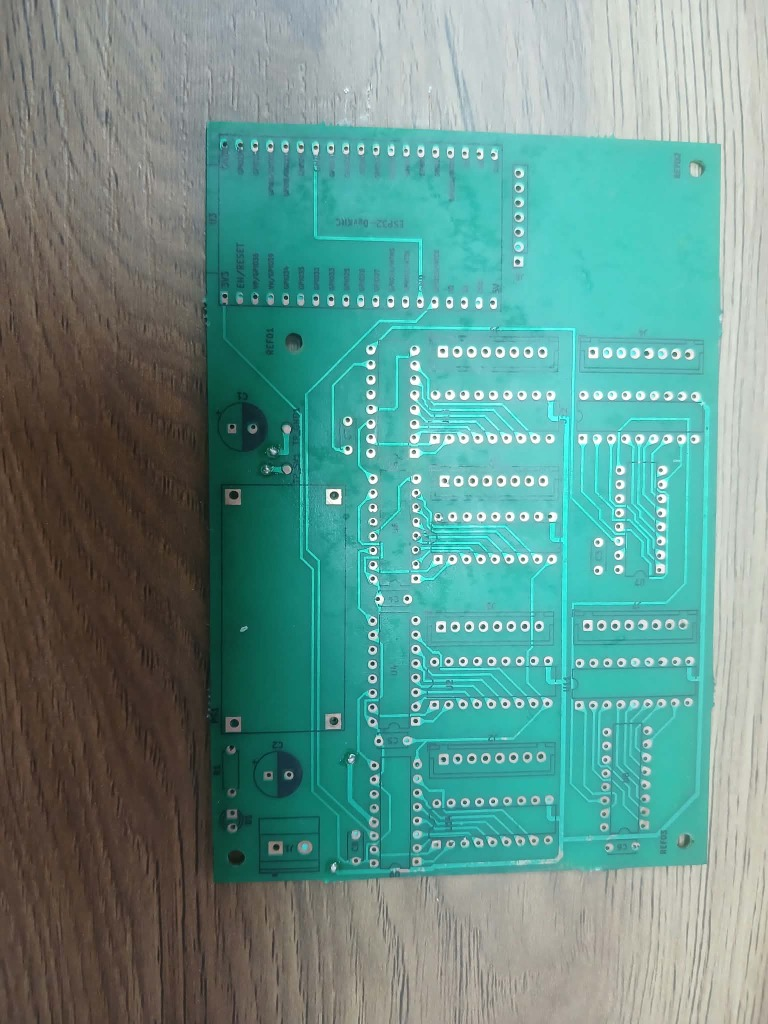
\includegraphics[width=\textwidth]{figures/real_pcb_top.jpg}
    \caption{Component side (F.Cu) with silkscreen outlines}
\end{subfigure}
\hfill
\begin{subfigure}[b]{0.48\textwidth}
    \centering
    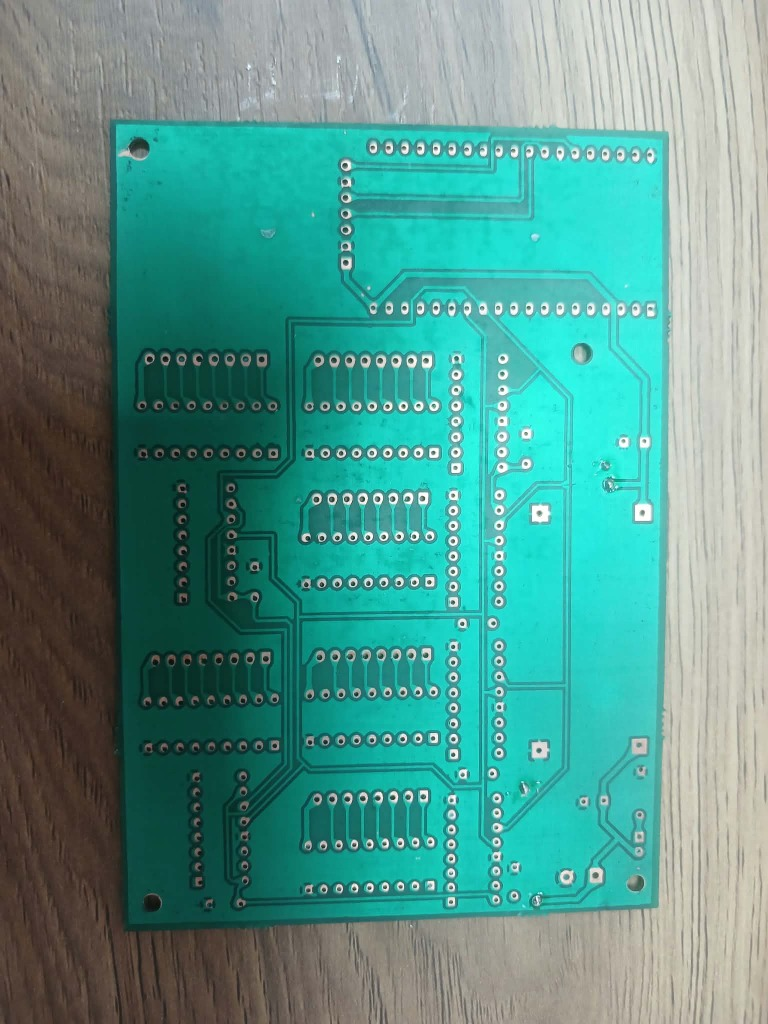
\includegraphics[width=\textwidth]{figures/real_pcb_bottom.jpg}
    \caption{Solder side (B.Cu) showing manual chemical etching}
\end{subfigure}
\caption{Physical Double-Sided Fabricated PCB of CHRONO\_01 (Chemical Etching Rapid-Prototyping)}
\label{fig:real_pcb}
\end{figure}



\subsection{Design Rule Check (DRC) and Thermal Performance}
Final automated DRC execution under KiCad confirmed **0 Errors and 0 Warnings**. Under full continuous illumination load (\texttt{88:88:88} at $24\,\text{V}$, drawing $1.68\,\text{A}$ for over 4 hours):
\begin{itemize}
    \item The ULN2803A Darlington drivers stabilized at a case temperature of $T_c \approx 42^\circ\text{C}$ (well below the $150^\circ\text{C}$ junction maximum).
    \item The LM2596 switching regulator maintained an operating temperature of $T_c \approx 38^\circ\text{C}$.
\end{itemize}

% ==============================================================================
% CHAPTER 5: FUTURE PERSPECTIVES & SYSTEM UPGRADES
% ==============================================================================
\chapter{Future Perspectives and System Upgrades}

\section{Introduction}
While the \textbf{CHRONO\_01} platform fulfills all functional criteria defined in the initial specifications, industrial hardware must be designed with scalability and future-proofing in mind. This chapter outlines planned hardware, communications, and power enhancements.

\section{4G LTE-Cat1 Cellular Migration (A7670C / SIM7000G)}
With telecommunication operators globally phasing out 2G GSM networks ("2G Sunset"), transitioning the cellular stage to modern 4G LTE is an essential long-term upgrade.

\begin{table}[H]
\centering
\small
\caption{Cellular Module Migration Comparison}
\label{tab:gsm_upgrade}
\begin{tabularx}{\textwidth}{>{\raggedright\arraybackslash}X c >{\raggedright\arraybackslash}p{4.5cm}}
\toprule
\textbf{Parameter} & \textbf{Current: SIM800L} & \textbf{Future Upgrade: SIMCom A7670C} \\
\midrule
Network Technology & 2G GSM / GPRS & \textbf{4G LTE-Cat1 / GSM Fallback} \\
Downlink / Uplink Data Rate & $85.6\,\text{kbps}$ & \textbf{$10\,\text{Mbps}$ / $5\,\text{Mbps}$} \\
Operating Voltage & $3.7\,\text{V} - 4.2\,\text{V}$ (Strict) & \textbf{$3.4\,\text{V} - 4.2\,\text{V}$ (Wide tolerance)} \\
Peak Burst Current & Up to $2.0\,\text{A}$ & \textbf{$\le 0.8\,\text{A}$ (Much lower peak)} \\
Footprint Compatibility & 2.54mm DIP Header & \textbf{Pin-Compatible Drop-In Variant} \\
Cloud Protocol Support & Basic HTTP & \textbf{Native MQTT, SSL/TLS, WebSockets} \\
\bottomrule
\end{tabularx}
\end{table}

\noindent Because the module was mounted using female header sockets on the PCB, upgrading to the 4G A7670C requires zero hardware modifications or PCB respins.

\section{Automotive Wide-Input SEPIC Power Supply Integration}
For mobile rally vehicle deployments (where the scoreboard is mounted on a car roof), vehicle battery voltage fluctuates widely:
\begin{itemize}
    \item Nominal battery voltage: $12.0\,\text{V} - 14.4\,\text{V}$.
    \item Cold-cranking engine starts: Dips down to $8.0\,\text{V}$.
    \item Load-dump overvoltage spikes: Up to $35\,\text{V}$.
\end{itemize}
A future PCB revision will integrate an on-board **SEPIC (Single-Ended Primary-Inductor Converter)** regulator. A SEPIC converter can step voltage up or down seamlessly, converting any input from $9\,\text{V}$ to $36\,\text{V}$ into a rock-solid, regulated $24.0\,\text{V}$ output.

\section{Cloud Telemetry and NTP Time Synchronization}
By connecting the ESP32 to local track WiFi or 4G data, the chronometer can synchronize with global atomic clocks via **Network Time Protocol (NTP)**, achieving microsecond-accurate timekeeping without requiring external RTC hardware. Furthermore, race splits can be streamed to cloud databases (Firebase, MQTT) for live online leaderboard viewing.

% ==============================================================================
% GENERAL CONCLUSION
% ==============================================================================
\chapter*{General Conclusion}
\addcontentsline{toc}{chapter}{General Conclusion}

\section*{Summary of Achievements}
The \textbf{CHRONO\_01} project represents an end-to-end engineering success spanning electrical theory, computer-aided PCB design, fabrication problem-solving, embedded firmware programming, and physical prototype assembly:
\begin{itemize}
    \item \textbf{Theoretical \& Sizing Analysis:} Derived the differential equations governing GSM peak current transient buffering ($C_1 = 1000\,\mu\text{F}$) and Buck regulator filter ripple suppression ($C_2 = 100\,\mu\text{F}$).
    \item \textbf{High-Density PCB Optimization:} Compacted the board footprint by $58.4\%$ through an orthogonal T-shape modular topology while resolving all NPTH rapid-prototyping constraints via machined-pin tulip sockets and teardrop fillets.
    \item \textbf{Full-Stack Prototyping:} Successfully integrated an ESP32 asynchronous Soft-AP Web server with hardware SPI shifting and cellular AT SMS parsing.
    \item \textbf{Optical \& Mechanical Engineering:} Built a rugged, high-contrast 6-digit display enclosure with optical baffles and PMMA opal diffusion.
\end{itemize}

\section*{Concluding Remarks}
This project demonstrates that high-performance, industrial-grade embedded hardware can be designed, optimized, and manufactured locally using rigorous engineering methodologies. The resulting platform delivers a versatile, robust timing instrument suitable for immediate athletic field deployment.

\newpage

% ------------------------------------------------------------------------------
% REFERENCES
% ------------------------------------------------------------------------------
\begin{thebibliography}{99}
\addcontentsline{toc}{chapter}{References}

\bibitem{esp32} Espressif Systems, \emph{ESP32-WROVER-E Datasheet and Technical Reference Manual}, v1.4, 2023.
\bibitem{74hc595} Texas Instruments, \emph{SN74HC595 8-Bit Shift Registers With 3-State Output Registers}, SCLS041I, 2022.
\bibitem{uln2803a} STMicroelectronics, \emph{ULN2803A Eight Darlington Transistor Array Datasheet}, DocID5279 Rev 8, 2018.
\bibitem{sim800l} SIMCom Wireless Solutions, \emph{SIM800L Hardware Design Manual}, v1.07, 2020.
\bibitem{ipc2152} IPC Association, \emph{IPC-2152: Standard for Determining Current-Carrying Capacity in Printed Board Design}, 2009.
\bibitem{kicad} KiCad PCB Design Software, \emph{KiCad 10 Reference Manual}, Open Source, 2026.

\end{thebibliography}

% ------------------------------------------------------------------------------
% APPENDIX
% ------------------------------------------------------------------------------
\appendix
\chapter{Technical Reference and Bill of Materials}

\section{Complete Bill of Materials (BOM)}
\begin{table}[H]
\centering
\footnotesize
\caption{CHRONO\_01 Final Component Bill of Materials}
\label{tab:bom}
\begin{tabularx}{\textwidth}{c c >{\raggedright\arraybackslash}X >{\raggedright\arraybackslash}p{4.5cm}}
\toprule
\textbf{Qty} & \textbf{Ref.} & \textbf{Component Description} & \textbf{Package / Spec} \\
\midrule
1  & $U_3$                               & ESP32-WROVER-E Microcontroller Board        & 38-Pin DevKitC Module \\
2  & $HDR_{1,2}$                         & Female Socket Headers for ESP32             & 1×19 Pin, 2.54 mm \\
6  & $U_{4-9}$                           & 74HC595 8-Bit Shift Register IC             & DIP-16 Through-Hole \\
6  & $SKT_{1-6}$                         & Machined-Pin Tulip Sockets for 74HC595      & DIP-16 Tulip (Elevated) \\
6  & $U_{10-14,U_2}$                     & ULN2803A Darlington Transistor Array        & DIP-18 Through-Hole \\
6  & $SKT_{7-12}$                        & Machined-Pin Tulip Sockets for ULN2803A    & DIP-18 Tulip (Elevated) \\
1  & $PS_1$                              & LM2596 Step-Down Buck Converter             & 24V → 5V DC-DC Module \\
1  & $MOD_1$                             & SIM800L Cellular GSM Transceiver           & Quad-Band Breakout \\
1  & $C_1$                               & Buffer Electrolytic Capacitor               & 1000 µF / 16 V Low-ESR \\
1  & $C_2$                               & Input Filter Electrolytic Capacitor         & 100 µF / 50 V Radial \\
6  & $C_{3,5,6,7,8,\text{dec}}$          & Decoupling Ceramic Capacitors               & 100 nF / 50 V \\
1  & $R_1$                               & Power LED Current Limiting Resistor         & 2.4 k$\Omega$ / 0.25 W Metal Film \\
1  & $D_1$                               & Power Indicator LED                         & 5 mm High-Efficiency Red \\
1  & $J_1$                               & Main 24V DC Power Input Connector           & 2-Pin Screw Terminal 5.08 mm \\
6  & $J_{2-7}$                           & Digit Segment Output Connectors             & JST-XH 8-Pin Male 2.54 mm \\
1  & $Conn\_01x07$                       & GSM / Expansion Header                      & 7-Pin Header 2.54 mm \\
2  & $TP_{1,2}$                          & Hardware Diagnostic Test Points             & 5V and GND Test Loops \\
42 & $SEG_{1-42}$                        & High-Intensity 24V COB LED Strip Bars       & 12 cm COB Strip (24V DC) \\
1  & $DIFF_1$                            & Front Optical Diffusion Panel               & 3 mm Opal White PMMA \\
\bottomrule
\end{tabularx}
\end{table}


\end{document}
